\documentclass[a4paper]{article}

\usepackage[english]{babel}
\usepackage[utf8]{inputenc}
\usepackage{csquotes}
\usepackage{amsmath, latexsym}
\usepackage{graphicx}
\usepackage{tikz}
\usepackage{listings}
\usepackage{verbatim}
\usepackage{bigints}
\usepackage{float}
\usepackage{titling}
\usepackage[colorinlistoftodos]{todonotes}
\usepackage[style=authoryear,sorting=nty,maxcitenames=1]{biblatex}



\title{Implementation of Kirchhoff acoustic solver}
\author{Magu Raam Prasaad R}
\date{\today}
\addbibresource{references.bib}



\begin{document}
\maketitle                                                                                                
\section{Mathematical formulation}
\begin{figure}[h!]\label{Kirchhoff}
	\centering
	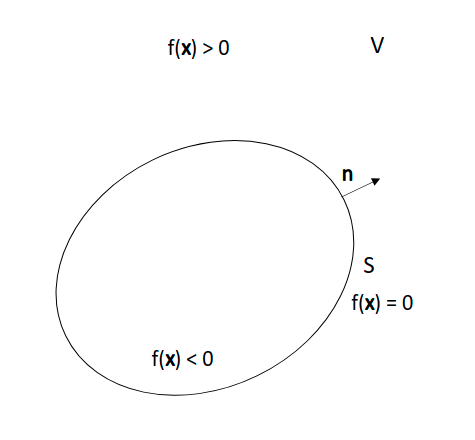
\includegraphics[width=60mm]{images/kirchhoff_surface.png}
	\caption{Stationary Kirchhoff surface $S$ encloses sound source}
\end{figure}
In this section, we derive the Kirchhoff formula for a stationary control surface (\cite{FARASSAT1988451}). We chose a control surface $S$ that encloses all the acoustic sources (\ref{Kirchhoff}), and the pressure perturbations $p$ satisfies the homogeneous wave equation 
\begin{equation}\label{Wave equation}
	\Bigg( \frac{1}{c_{0}^2}\frac{\partial{}^{2}}{\partial{t}^{2}}- \nabla{}^{2} \Bigg) p = 0 \quad \quad \textrm{in} \ V. 
\end{equation}
The control surface S is defined by $f(\mathbf{x}) = 0$, $f(\mathbf{x}) > 0$ for $\mathbf{x}$ in V and $f(\mathbf{x}) < 0$ for $\mathbf{x}$ inside surface S. We scale the function $f$ such that $\nabla f = \mathbf{n}$. Then the Heaviside function of $f(\mathbf{x})$    is
\begin{equation}\label{Heaviside}
	H(f) =\begin{cases}
	1, & \text{for $\mathbf{x}$ in V}.\\
	0, & \text{for $\mathbf{x}$ inside S}.
	\end{cases}
\end{equation}
The gradient of the Heaviside function is given by
\begin{equation}\label{Gradient Heaviside}
	\nabla H(f) = \delta (f) \mathbf{n}.
\end{equation}
We define the pressure $p$ as a generalized function $pH(f)$ (\cite{ffowcs1969sound}) where
\begin{equation}\label{Generalized_Functions}
	p H(f) =\begin{cases}
	p , & \text{for $\mathbf{x}$ in V}.\\
	0, & \text{for $\mathbf{x}$ inside S}.
	\end{cases}
\end{equation}
The generalized pressure $pH(f)$ is defined everywhere in space, unlike $p$ defined only in $V$. We will derive the acoustic wave equation for the generalised pressure. Using (\ref{Gradient Heaviside}), the gradient of $pH$ is
\begin{equation}
	\nabla (pH) = \nabla p H + p \delta(f)\mathbf{n}.
\end{equation}
Therefor the Laplacian is given by
\begin{equation}\label{Laplacian}
	\nabla^2 (pH) = \nabla^2 p H +  \frac{\partial p}{\partial n}\delta(f) + \nabla.(p \delta(f)\mathbf{n}).
\end{equation}
The partial derivative in time is
\begin{equation}\label{Time derivative}
	\frac{\partial^2}{\partial t^2}(pH) = \frac{\partial^2 p }{\partial t^2}H.
\end{equation}
We premultiply (\ref{Time derivative}) with $1/{c_{0}^2}$ and subtract (\ref{Laplacian}) to obtain the acoustic wave equation in generalised pressure
\begin{equation}
	\Bigg( \frac{1}{c_{0}^2}\frac{\partial{}^{2}}{\partial{t}^{2}}- \nabla{}^{2} \Bigg) pH = H\Bigg( \frac{1}{c_{0}^2}\frac{\partial{}^{2}}{\partial{t}^{2}}- \nabla{}^{2} \Bigg) p - \frac{\partial p}{\partial n}\delta(f) - \nabla.(p \delta(f)\mathbf{n}), 
\end{equation}
or
\begin{equation}\label{Generalized Wave Equation}
	\Bigg( \frac{1}{c_{0}^2}\frac{\partial{}^{2}}{\partial{t}^{2}}- \nabla{}^{2} \Bigg) pH = -\frac{\partial p}{\partial n}\delta(f) - \nabla.(p \mathbf{n} \delta(f)). 
\end{equation}
The right side of the equation (\ref{Generalized Wave Equation}) is non-zero only at surface $S$, as it contains $\delta (f)$. The acoustic wave equation (\ref{Generalized Wave Equation}) in generalized variables is valid in the entire unbounded space. Therefore we can use free-space Green's function to solve the equation. The Green's function is the solution of wave equation for an impulsive point source $\delta(\mathbf{x} - \mathbf{y})\delta(t - \tau)$ placed at point $\mathbf{y}$ and time $\tau$
\begin{equation}\label{green}
	\Bigg( \frac{1}{c_{0}^2}\frac{\partial{}^{2}}{\partial{t}^{2}}- \nabla{}^{2} \Bigg){G(\mathbf{x}, t; \mathbf{y}, \tau )} = \delta{(\mathbf{x} - \mathbf{y})}\delta{(t - \tau)}. 
\end{equation}
The Green's function for the acoustic wave operator (\cite{howe2003theory}) in three dimensions is
\begin{equation}\label{Green's Function}
	G(\mathbf{x}, t; \mathbf{y}, \tau ) = \frac{\delta \Big(t - \tau - \frac{|\mathbf{x} - \mathbf{y}|}{c_{0}}\Big)}{4\pi|\mathbf{x} - \mathbf{y}|}.
\end{equation}
The solution for arbirtary source can be obtained by multiplying $s(\mathbf{y}, \tau)$ in (\ref{green})
\begin{equation}
	\Bigg( \frac{1}{c_{0}^2}\frac{\partial{}^{2}}{\partial{t}^{2}}- \nabla{}^{2} \Bigg)s(\mathbf{y}, \tau){G(\mathbf{x}, t; \mathbf{y}, \tau )} = s(\mathbf{y}, \tau)\delta{(\mathbf{x} - \mathbf{y})}\delta{(t - \tau)}, 
\end{equation}
Integrating both sides
\begin{equation}
	\Bigg( \frac{1}{c_{0}^2}\frac{\partial{}^{2}}{\partial{t}^{2}}- \nabla{}^{2} \Bigg) \int s(\mathbf{y}, \tau){G(\mathbf{x}, t; \mathbf{y}, \tau )} d\mathbf{y}d\tau  = \int s(\mathbf{y}, \tau)\delta{(\mathbf{x} - \mathbf{y})}\delta{(t - \tau)} d\mathbf{y}d\tau,  
\end{equation}
and using the properties of delta function, we get the solution for the acoustic wave equation with source $s(\mathbf{x}, t)$
\begin{equation}
	\Bigg( \frac{1}{c_{0}^2}\frac{\partial{}^{2}}{\partial{t}^{2}}- \nabla{}^{2} \Bigg) p(\mathbf{x}, t)  = s(\mathbf{x}, t), 
\end{equation}
where,
\begin{equation}\label{pressure}
	p(\mathbf{x}, t) = \int s(\mathbf{y}, \tau){G(\mathbf{x}, t; \mathbf{y}, \tau )} d\mathbf{y}d\tau. 
\end{equation}
We can use the above relation to solve the acoustic wave equation (\ref{Generalized Wave Equation})
\begin{equation}
	\begin{split}
		(pH)(\mathbf{x}, t) = &-\frac{1}{4\pi}\int {\frac{\partial p}{\partial n}\delta(f) \frac{\delta \Big(t - \tau - \frac{|\mathbf{x} - \mathbf{y}|}{c_{0}}\Big)}{|\mathbf{x} - \mathbf{y}|}} d\mathbf{y}d\tau \\
		&-\frac{1}{4\pi}\int \nabla_{\mathbf{y}}.(p \mathbf{n} \delta(f)){\frac{\delta \Big(t - \tau - \frac{|\mathbf{x} - \mathbf{y}|}{c_{0}}\Big)}{|\mathbf{x} - \mathbf{y}|}} d\mathbf{y}d\tau.
	\end{split}
\end{equation}
Incomplete step!
\begin{equation}
	\begin{split}
		(pH)(\mathbf{x}, t) = &-\frac{1}{4\pi}\int {\frac{\partial p}{\partial n}\delta(f) \frac{\delta \Big(t - \tau - \frac{|\mathbf{x} - \mathbf{y}|}{c_{0}}\Big)}{|\mathbf{x} - \mathbf{y}|}} d\mathbf{y}d\tau \\
		&-\frac{1}{4\pi}\nabla_{\mathbf{x}}.\int (p \mathbf{n} \delta(f)){\frac{\delta \Big(t - \tau - \frac{|\mathbf{x} - \mathbf{y}|}{c_{0}}\Big)}{|\mathbf{x} - \mathbf{y}|}} d\mathbf{y}d\tau.
	\end{split}
\end{equation}
We use the following property to convert volume integral to surface integral (\cite{FARASSAT1988451}).
Incomplete step !
\begin{equation}\label{volume surface}
	\int \phi (\mathbf{y}) \delta (f) \mathbf{n} d\mathbf{y} = \int_{S} \phi (\mathbf{y}) \mathbf{n} dS
\end{equation}
We use the above property to convert volume integral to surface integral on $S$
\begin{equation}
	\begin{split}
		(pH)(\mathbf{x}, t) = &-\frac{1}{4\pi}\int {\frac{\partial p}{\partial n} \frac{\delta \Big(t - \tau - \frac{|\mathbf{x} - \mathbf{y}|}{c_{0}}\Big)}{|\mathbf{x} - \mathbf{y}|}} dSd\tau \\
		&-\frac{1}{4\pi}\nabla_{\mathbf{x}}.\int (p \mathbf{n} ){\frac{\delta \Big(t - \tau - \frac{|\mathbf{x} - \mathbf{y}|}{c_{0}}\Big)}{|\mathbf{x} - \mathbf{y}|}} dSd\tau.
	\end{split}
\end{equation}
Using the property of delta function we obtain
\begin{equation}
	\begin{split}
		(pH)(\mathbf{x}, t) = &-\frac{1}{4\pi}\int_{S} { \Big[\frac{\partial p}{\partial n}\Big] \frac{dS}{|\mathbf{x} - \mathbf{y}|}}  \\
		&-\frac{1}{4\pi}\nabla_{\mathbf{x}}.\int_{S} [p]\mathbf{n}{\frac{dS}{|\mathbf{x} - \mathbf{y}|}} .
	\end{split}
\end{equation}
The square bracket implies the functions are computed at the retarded time i.e, $[p] = p(\mathbf{y}, t - \frac{|\mathbf{x} - \mathbf{y}|}{c})$. Simplifying the equation further, we obtain the \textbf{Kirchhoff formula} for a stationary control surface (\cite{FARASSAT1988451}, \cite{jamaluddin}).
\begin{equation}\label{Kirchhoff Integral}
	\begin{split}
		(pH)(\mathbf{x}, t) = -\frac{1}{4\pi}\int_{S}\Big[  \frac{p}{r^{2}}\frac{\partial r}{\partial n} - \frac{1}{r}\frac{\partial p}{\partial n} + \frac{1}{c r}\frac{\partial r}{\partial n}\frac{\partial p}{\partial \tau} \Big]_{\tau} dS.
	\end{split}
\end{equation}
Where, $r = |\mathbf{x} - \mathbf{y}|$, the square bracket again implies the functions are computed at the retarded time $\tau = t - r/c$.
\section{Results}
We compute the sound waves emitted by a monopole source using the Kirchhoff solver. The acoustic wave equation for a monopole source placed at a point $\mathbf{x} = 0$ is
\begin{equation}
	\Bigg( \frac{1}{c_{0}^2}\frac{\partial{}^{2}}{\partial{t}^{2}}- \nabla{}^{2} \Bigg) p(\mathbf{x}, t)  = -q(t)\delta(\mathbf{x}), 
\end{equation}
where $q(t)$ is the time dependent source function. The solution can be obtained by substituting the free space Green's function (\ref{Green's Function}) in (\ref{pressure})
\begin{equation}
	p(\mathbf{x}, t) = \int s(\mathbf{y}, \tau) \frac{1}{4\pi|\mathbf{x} - \mathbf{y}|}\delta \Bigg(t - \tau - \frac{|\mathbf{x} - \mathbf{y}|}{c_{0}}\Bigg)d\mathbf{y}d\tau, 
\end{equation}
and using the property of delta function we obtain,
\begin{equation}\label{retarded potential}
	p(\mathbf{x}, t) = \frac{1}{4\pi}\int \frac{s\Big(\mathbf{y}, t - \frac{|\mathbf{x} - \mathbf{y}|}{c_{0}}\Big)}{|\mathbf{x} - \mathbf{y}|}d\mathbf{y}. 
\end{equation}
The pressure at any point $\mathbf{x}$ and time $t$ is a linear superposition of contributions from all the sources located at $\mathbf{y}$, which radiated at the earliest times $t - \frac{|\mathbf{x} - \mathbf{y}|}{c_{0}}$. The integral formula (\ref{retarded potential}) is called the retarded potential. Substituting $s(\mathbf{y}, \tau) = -q(t)\delta(\mathbf{x})$ in the above equation we obtain
\begin{equation}
	p(\mathbf{x}, t) = -\frac{1}{4\pi}\int \frac{ \delta (\mathbf{y}) q(t - \frac{|\mathbf{x} - \mathbf{y}|}{c_{0}}) }{{|\mathbf{x} - \mathbf{y}|}}d\mathbf{y},
\end{equation}
using the property of delta function, the pressure radiated by a monopole source is given by
\begin{equation}
	p(\mathbf{x}, t) = -\frac{1}{4\pi} \frac{  q(t - \frac{r}{c_{0}}) }{r}. 
\end{equation}
where $r = {|\mathbf{x}|}$.
\subsection{Monopole test case}
We chose the monopole of strength
\begin{equation}
	q(t) = 2(t - t0)f_{0}^{2}\exp( -f_{0}^2(t - t_{0})^{2}). 
\end{equation}
where $f_{0} = 100$ is the dominant frequency and $t_{0} = \frac{4}{f_{0}}$.
\begin{figure}[h!]\label{Monopole}
	\centering
	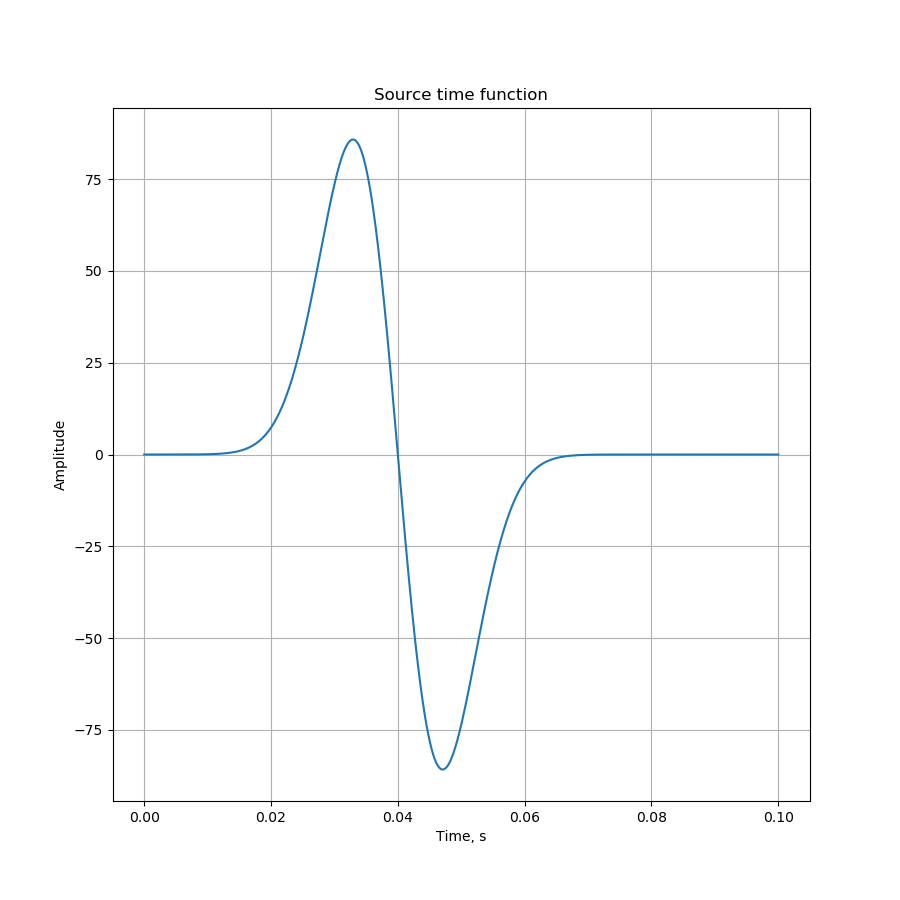
\includegraphics[width=80mm]{images/Source.png}
	\caption{Monopole source as a function of time}
\end{figure}
We enclose the monopole source using a cuboidal Kirchhoff surface whose diagonally opposite points are $p_{1} = (-1.0, -1.0, -1.0)$
and $p_{2} = (1.0, 1.0, 1.0)$. The surface is embedded in a cuboidal domain of size $[-5.0,5.0]\times[-5.0,5.0]\times[-5.0,5.0]$. The domain is discretized into structured grid of size $h = 0.1$ and the Kirchhoff surface is discretized into square cells of size $h = 0.1$. The pressure and its derivatives are interpolated from cell centers to quadrature points on Kirchhoff surface using fourth-order WENO polynomial. The Kirchhoff Integral (\ref{Kirchhoff Integral}) is computed using the two-point Gauss quadrature formula. The exact and numerical pressure are evaluated at observer point $xo = (3.0,3.0,3.0)$ and plotted against the function of time.
\begin{figure}[h!]\label{Result}
	\centering
	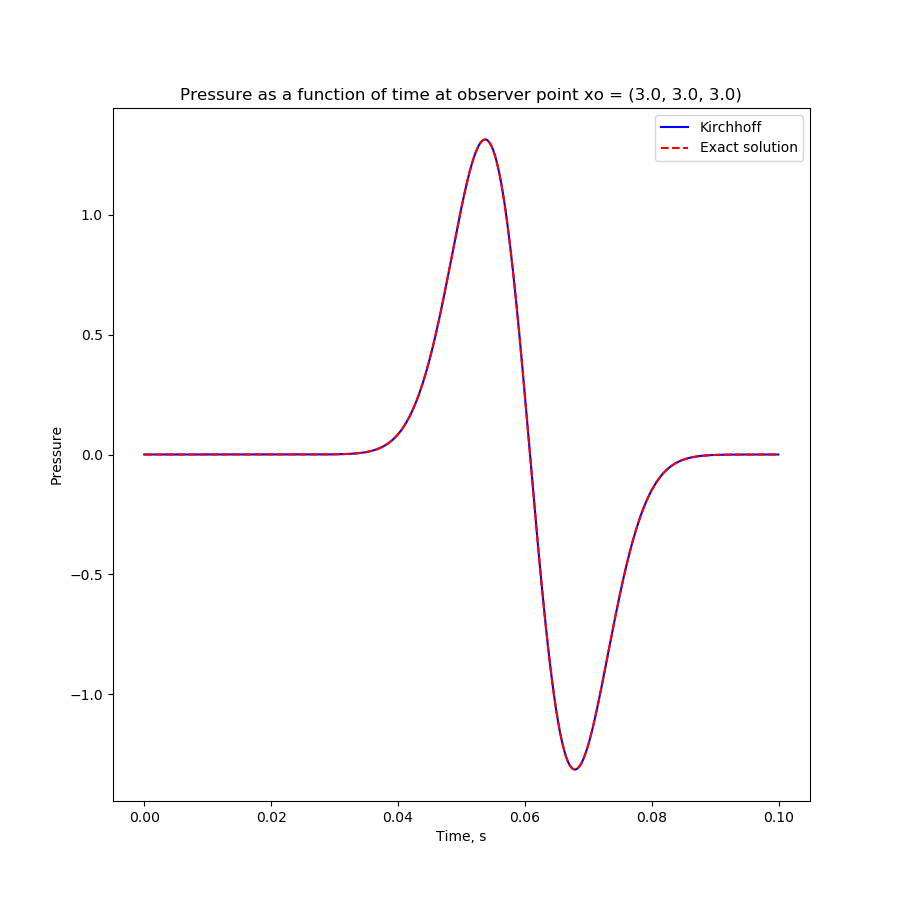
\includegraphics[width=80mm]{images/Pressure.png}
	\caption{The exact and numerical pressure as a function of time at observer point $xo = (3.0,3.0,3.0)$.The $L_{\infty}$ error is 3.11e-4.} 
\end{figure}

\printbibliography
\end{document}
 
